\chapter{Pruebas y Resultados}
\label{chap:resultados}

En este capítulo se presenta la evaluación experimental del \textit{pipeline} liviano propuesto. Los experimentos se organizan en torno a los objetivos específicos del trabajo: (i) cuantificar la brecha del \textit{pipeline} liviano frente a los \textit{Teachers} \ac{I3D} y SlowFast-R50 en tres dominios (\textbf{OE3}); (ii) caracterizar la eficiencia computacional del \textit{pipeline} (\textbf{OE5}); (iii) aislar el aporte de los componentes clave mediante ablaciones (\textbf{OE4}); y (iv) delimitar los límites de aplicabilidad mediante transferencia cruzada y un análisis marginal de la destilación de conocimiento (\textbf{OE6}).

\section{Comparación principal: pipeline liviano frente a Teachers}
\label{sec:comparacion_principal}

La Tabla~\ref{tab:precision_aqa7} reporta la comparación principal en AQA-7, el dataset principal del trabajo. Los \textit{Students} se ejecutan con tres semillas aleatorias (42, 0 y 7) y se reporta media $\pm$ desviación estándar. Los \textit{Teachers} \ac{I3D} y SlowFast-R50 se ejecutan con semilla 42.

\begin{table}[H]
\centering
\caption{Resultados de precisión en AQA-7. Los \textit{Students} (\textit{Pipeline liviano}) se ejecutan con tres semillas (42, 0 y 7) y se reporta media $\pm$ desviación estándar; los \textit{Teachers} y las variantes \textit{+~KD} se ejecutan con semilla 42. La columna \textit{Régimen} distingue: \textit{Teacher} = referencia 3D; \textit{Pipeline liviano} = propuesta principal; \textit{+~KD} = análisis marginal con destilación activa.}
\label{tab:precision_aqa7}
\small
\begin{tabular}{llccc}
\toprule
\textbf{Modelo} & \textbf{Régimen} & \textbf{SRCC}↑ & \textbf{PLCC}↑ & \textbf{MAE}↓ \\
\midrule
SlowFast-R50      & Teacher (3D moderno)   & \textbf{0.9158}              & ---    & ---  \\
I3D-R50           & Teacher (3D histórico) & 0.9052                       & 0.9352 & 8.20 \\
\midrule
TSM-MobileNetV2   & Pipeline liviano       & $\mathbf{0.9021 \pm 0.0046}$ & 0.9356 & 8.67 \\
MobileNetV3       & Pipeline liviano       & $\mathbf{0.8907 \pm 0.0049}$ & 0.9271 & 9.32 \\
\midrule
TSM-MobileNetV2   & + KD                   & 0.8811                       & 0.9299 & 8.40 \\
MobileNetV3       & + KD                   & 0.9250                       & 0.9561 & 6.15 \\
\bottomrule
\end{tabular}
\end{table}

\paragraph{Brecha frente a Teachers.} La Tabla~\ref{tab:precision_aqa7} muestra que el \textit{pipeline} liviano cierra la brecha con los \textit{Teachers} 3D a una distancia muy reducida:

\begin{itemize}
    \item TSM-MobileNetV2 (media $0.9021$) queda a $-0.003$ \ac{SRCC} del \ac{I3D} (0.9052) y a $-0.014$ \ac{SRCC} del SlowFast-R50 (0.9158).
    \item MobileNetV3 (media $0.8907$) queda a $-0.014$ \ac{SRCC} del \ac{I3D} y a $-0.025$ \ac{SRCC} del SlowFast-R50.
\end{itemize}

La inclusión de SlowFast-R50 como \textit{Teacher} 3D moderno permite afirmar que la cercanía del \textit{pipeline} liviano no es sólo respecto al baseline histórico (\ac{I3D}, 2017), sino también respecto al estado actual del paradigma 3D. Las desviaciones estándar bajas ($\sim 0.005$ en ambos \textit{Students}) confirman que el resultado no depende de una inicialización favorable.

La Tabla~\ref{tab:precision_otros} reporta los resultados en los otros dos datasets (semilla 42), donde se evalúan los mismos modelos sin réplicas adicionales por costo computacional.

\begin{table}[H]
\centering
\caption{Resultados de precisión en MTL-AQA y JIGSAWS (semilla 42). Se incluyen los regímenes \textit{Pipeline liviano} (sólo $\mathcal{L}_{reg}$) y \textit{+~KD} (análisis marginal).}
\label{tab:precision_otros}
\small
\begin{tabular}{llcccc}
\toprule
\textbf{Modelo} & \textbf{Régimen} & \textbf{Dataset} & \textbf{SRCC}↑ & \textbf{PLCC}↑ & \textbf{MAE}↓ \\
\midrule
I3D             & Teacher          & MTL-AQA & \textbf{0.8869} & 0.8848          & \textbf{5.51}  \\
TSM-MobileNetV2 & Pipeline liviano & MTL-AQA & 0.8804          & 0.8697          & 6.06           \\
TSM-MobileNetV2 & + KD             & MTL-AQA & 0.7628          & 0.7564          & 8.42           \\
MobileNetV3     & Pipeline liviano & MTL-AQA & 0.8703          & \textbf{0.8744} & 6.06           \\
MobileNetV3     & + KD             & MTL-AQA & 0.8470          & 0.8288          & 7.43           \\
\midrule
I3D             & Teacher          & JIGSAWS & 0.8364          & \textbf{0.8456} & \textbf{10.83} \\
TSM-MobileNetV2 & Pipeline liviano & JIGSAWS & 0.8283          & 0.8007          & 11.76          \\
TSM-MobileNetV2 & + KD             & JIGSAWS & 0.3435          & 0.3428          & 20.57          \\
MobileNetV3     & Pipeline liviano & JIGSAWS & \textbf{0.8368} & 0.8356          & 10.31          \\
MobileNetV3     & + KD             & JIGSAWS & 0.7907          & 0.7777          & 11.52          \\
\bottomrule
\end{tabular}
\end{table}

En MTL-AQA y JIGSAWS la brecha SRCC entre el \textit{pipeline} liviano y el \textit{Teacher} es nuevamente menor a 0.01 ($-0.007$ y $-0.008$ respectivamente), consistente con lo observado en AQA-7. Esto sostiene la afirmación central del trabajo: el \textit{pipeline} liviano moderno no es una solución aislada para un único dataset, sino una alternativa estable en dominios de naturaleza distinta (deporte multi-disciplina, clavados especializados, cirugía robótica).

\section{Eficiencia computacional}
\label{sec:eficiencia}

La Tabla~\ref{tab:eficiencia} reporta el número de parámetros, los \ac{FLOPs} (calculados con \texttt{fvcore}) y la latencia mediana de inferencia (\textit{batch~1}, $T=64$, $H=W=224$) sobre una NVIDIA RTX 3060 Mobile (6~GB de VRAM).

\begin{table}[H]
\centering
\caption{Eficiencia computacional. Latencia mediana sobre RTX 3060 Mobile (mediana sobre 20 corridas), \textit{batch}~1, clip $T=64$. Se incluye X3D-M como Student 3D liviano adicional.}
\label{tab:eficiencia}
\small
\begin{tabular}{lccc}
\toprule
\textbf{Modelo} & \textbf{Params (M)}↓ & \textbf{FLOPs (G)}↓ & \textbf{Latencia (ms)}↓ \\
\midrule
SlowFast-R50    & 33.65        & 101.2         & 88.9           \\
I3D-R50         & 27.23        & 228.3         & 140.8          \\
\midrule
X3D-M           & \textbf{2.01} & 19.3          & 62.6           \\
TSM-MobileNetV2 & 2.23         & 20.0          & 56.5           \\
MobileNetV2 plano (E7) & 2.23  & 20.0          & 54.0           \\
MobileNetV3     & 2.97         & \textbf{14.3} & \textbf{42.0}  \\
\bottomrule
\end{tabular}
\end{table}

Los \textit{Students} reducen los \ac{FLOPs} en más del $91\%$ frente al \textit{Teacher} \ac{I3D} (TSM-MobileNetV2: 20.0~G vs 228.3~G; MobileNetV3: 14.3~G), con parámetros aproximadamente $10\times$ menores y latencia entre $2.5$ y $3.4\times$ menor. MobileNetV3 alcanza 39.9~ms por clip de 64 \textit{frames}, lo que habilita aplicaciones en tiempo real en dispositivos embebidos. Este resultado, combinado con la brecha SRCC menor a $0.015$, valida que el \textit{pipeline} liviano no es sólo competitivo en precisión sino también drásticamente más eficiente.

\section{Ablaciones del pipeline}
\label{sec:ablaciones}

Para responder \textbf{OE4}, se ejecutaron dos ablaciones sobre AQA-7 (semilla 42, TSM-MobileNetV2) que aíslan el aporte de los componentes clave del \textit{pipeline}: el preentrenamiento ImageNet y el módulo temporal explícito.

\subsection{Ablación E6: aporte del preentrenamiento ImageNet}

La Tabla~\ref{tab:ablation_pretrain} compara TSM-MobileNetV2 con y sin pesos preentrenados de ImageNet. Sin preentrenamiento, el modelo se inicializa aleatoriamente y se entrena durante 80 \textit{epochs} (vs 50 del \textit{baseline}) para compensar la falta de inicialización fuerte.

\begin{table}[H]
\centering
\caption{Ablación E6 — aporte del preentrenamiento ImageNet en TSM-MobileNetV2 sobre AQA-7.}
\label{tab:ablation_pretrain}
\small
\begin{tabular}{lc}
\toprule
\textbf{Configuración} & \textbf{SRCC}↑ \\
\midrule
TSM-MBv2 con preentrenamiento ImageNet (media 3 semillas) & \textbf{0.9021} \\
TSM-MBv2 sin preentrenamiento (semilla 42) & 0.8713 \\
\midrule
$\Delta$ SRCC & $-0.031$ \\
\bottomrule
\end{tabular}
\end{table}

La caída de $0.031$ \ac{SRCC} ($\sim 3.4\%$ relativo) demuestra que el preentrenamiento ImageNet es un componente crítico del \textit{pipeline} propuesto. La transferencia de representaciones visuales aprendidas en ImageNet aporta una porción no trivial del cierre de brecha frente al \textit{Teacher}. Esto convierte la afirmación ``el \textit{pipeline} funciona'' en una más útil: el \textit{pipeline} funciona porque el preentrenamiento ImageNet aporta $\sim 3$ puntos de SRCC sobre el \textit{backbone} aleatorio.

\subsection{Ablación E7: aporte del componente temporal explícito (TSM)}

La Tabla~\ref{tab:ablation_tsm} compara TSM-MobileNetV2 (con \ac{TSM}) frente a una variante MobileNetV2 plana (sin \ac{TSM}, agregación temporal sólo por \textit{pooling} global), ambas inicializadas con pesos ImageNet.

\begin{table}[H]
\centering
\caption{Ablación E7 — aporte del módulo Temporal Shift sobre AQA-7 (semilla 42).}
\label{tab:ablation_tsm}
\small
\begin{tabular}{lc}
\toprule
\textbf{Configuración} & \textbf{SRCC}↑ \\
\midrule
TSM-MBv2 (con TSM, media 3 semillas) & \textbf{0.9021} \\
MobileNetV2 plano (sin TSM, semilla 42) & 0.8921 \\
\midrule
$\Delta$ SRCC & $-0.010$ \\
\bottomrule
\end{tabular}
\end{table}

La caída de $0.010$ \ac{SRCC} ($\sim 1.1\%$ relativo) indica que el módulo \ac{TSM} aporta un beneficio modesto pero positivo en AQA-7. Este resultado matiza la importancia del modelado temporal explícito: en datasets cuyas acciones son rápidas y bien caracterizadas por información espacial-instantánea (clavados, gimnasia, esquí), un \textit{pooling} temporal global ya captura la mayor parte de la señal. El componente temporal explícito sí aporta, pero su contribución es secundaria frente a la del preentrenamiento ImageNet (E6).

\paragraph{Síntesis de las ablaciones.} El \textit{pipeline} liviano se sostiene en dos componentes identificables y separables: (i) el preentrenamiento ImageNet moderno, responsable de $\sim 3$ puntos de \ac{SRCC}, y (ii) el módulo temporal eficiente \ac{TSM}, que añade $\sim 1$ punto adicional. La contribución de la tesis no se reduce a ``usar arquitectura liviana'', sino a usarla dentro de un \textit{pipeline} donde estos dos componentes están bien identificados.

\section{Frontera Pareto: precisión frente a costo computacional}
\label{sec:pareto}

Más allá de las comparaciones puntuales, una pregunta natural es: dado un presupuesto computacional, ¿qué arquitectura ofrece el mejor compromiso entre precisión y costo? La Tabla~\ref{tab:pareto} presenta la frontera Pareto en AQA-7 cruzando \ac{SRCC} con \ac{FLOPs}, parámetros y latencia, incluyendo el \textit{pipeline} liviano propuesto, sus ablaciones y la referencia 3D eficiente X3D-M.

\begin{table}[H]
\centering
\caption{Frontera Pareto en AQA-7. SRCC con semilla 42 (\textit{Students} 2D: media de 3 semillas; X3D-M: semilla 42). FLOPs y latencia tomados de la Tabla~\ref{tab:eficiencia}.}
\label{tab:pareto}
\small
\begin{tabular}{lcccc}
\toprule
\textbf{Modelo} & \textbf{Params (M)} & \textbf{FLOPs (G)} & \textbf{Latencia (ms)} & \textbf{SRCC}↑ \\
\midrule
SlowFast-R50    & 33.65 & 101.2     & 88.9   & 0.9158 \\
I3D-R50         & 27.23 & 228.3     & 140.8  & 0.9052 \\
\midrule
\textbf{X3D-M}  & \textbf{2.01} & \textbf{19.3} & 62.6  & \textbf{0.9211} \\
TSM-MobileNetV2 & 2.23  & 20.0      & 56.5   & 0.9021 \\
MobileNetV2 plano (E7) & 2.23 & 20.0 & 54.0  & 0.8921 \\
MobileNetV3     & 2.97  & 14.3      & 42.0   & 0.8907 \\
\bottomrule
\end{tabular}
\end{table}

De la Tabla~\ref{tab:pareto} se desprenden tres observaciones:

\begin{itemize}
    \item X3D-M \emph{domina la frontera Pareto absoluta}: alcanza \ac{SRCC} de $0.9211$ con apenas 19.3~GFLOPs, superando incluso a los \textit{Teachers} \ac{I3D} ($0.9052$, 228~G) y SlowFast-R50 ($0.9158$, 101~G), con menos del 20\% de los \ac{FLOPs} de SlowFast y menos del 9\% de los \ac{FLOPs} de \ac{I3D}.
    \item TSM-MobileNetV2 y MobileNetV3 quedan en la frontera de \ac{FLOPs} mínimos (20~G y 14~G respectivamente), a $\sim 0.02$ y $\sim 0.03$ \ac{SRCC} de X3D-M; útiles cuando el presupuesto computacional es aún más estricto.
    \item El hallazgo refuerza la hipótesis central del trabajo: la \emph{receta moderna de entrenamiento} (preentrenamiento, AdamW, cosine, AMP, gradient accumulation) eleva el techo de las arquitecturas livianas a un nivel donde superan a los modelos 3D pesados clásicos del campo, sin requerir destilación de conocimiento.
\end{itemize}

La conclusión práctica es que el \textit{pipeline} propuesto, instanciado en X3D-M, no sólo cierra la brecha frente a los \textit{Teachers} 3D sino que la invierte: con $\sim 9\%$ de los \ac{FLOPs} del \ac{I3D} alcanza un \ac{SRCC} $1.6\%$ superior. Esta inversión apoya la tesis empírica del trabajo: con prácticas modernas, las arquitecturas livianas son competitivas con o mejores que el SOTA 3D clásico en \ac{AQA} eficiente.

\section{Comparación con el estado del arte}
\label{sec:sota}

La Tabla~\ref{tab:sota} sitúa el \textit{pipeline} propuesto frente a métodos representativos del estado del arte reportados en la literatura reciente, en los dos benchmarks principales del campo (AQA-7 y MTL-AQA). Para los métodos previos se citan los \ac{SRCC} reportados en sus respectivos artículos.

\begin{table}[H]
\centering
\caption{Comparación con el estado del arte en AQA-7 y MTL-AQA. Los métodos previos usan mayoritariamente \ac{I3D} como \textit{backbone} (228+~GFLOPs); los métodos propuestos usan arquitecturas livianas (14--20~GFLOPs).}
\label{tab:sota}
\small
\begin{tabular}{lcccc}
\toprule
\textbf{Método} & \textbf{Año} & \textbf{SRCC AQA-7} & \textbf{SRCC MTL-AQA} & \textbf{FLOPs (G)} \\
\midrule
USDL \cite{Hinton2015Distilling}   & 2020 & 0.846 & 0.927 & $\sim$228 \\
GAKD \cite{Yu2021GroupAware}       & 2021 & $\sim$0.855 & --- & $\sim$228 \\
CoRe \cite{Yu2021GroupAware}       & 2021 & 0.840 & 0.951 & $\sim$250 \\
TSA-Net                            & 2021 & 0.848 & 0.939 & --- \\
TPT                                & 2022 & ---   & \textbf{0.961} & --- \\
HGCN                               & 2023 & 0.846 & 0.939 & --- \\
\midrule
MobileNetV3 (\textit{pipeline})     & 2026 & 0.891          & 0.870 & \textbf{14.3} \\
TSM-MobileNetV2 (\textit{pipeline}) & 2026 & 0.902          & 0.880 & 20.0 \\
\textbf{X3D-M (\textit{pipeline})}  & 2026 & \textbf{0.921} & ---   & 19.3 \\
\bottomrule
\end{tabular}
\end{table}

La lectura honesta de esta comparación es:

\begin{itemize}
    \item En \textbf{AQA-7}, las tres instancias del \textit{pipeline} propuesto superan a todos los métodos SOTA basados en \ac{I3D} reportados (USDL, GAKD, CoRe, TSA-Net, HGCN). En particular, X3D-M alcanza $0.921$ \ac{SRCC}, $6.5$ puntos por encima del mejor SOTA reportado en este dataset, usando $\sim 8.5\%$ de sus \ac{FLOPs}. Este resultado refuerza la tesis empírica: una receta moderna sobre arquitecturas livianas eleva el techo a un nivel donde los métodos con \textit{backbones} pesados clásicos pierden su ventaja.
    \item En \textbf{MTL-AQA}, los \textit{Students} 2D quedan aproximadamente 7--8 puntos por debajo del SOTA (TPT, CoRe). En este dataset especializado de clavados, los métodos SOTA incorporan componentes específicos (\textit{Temporal Parser}, regresión contrastiva, atención por grupos) que aportan en ese régimen pero requieren \textit{backbones} 3D pesados. La evaluación de X3D-M sobre MTL-AQA se identifica como dirección inmediata de trabajo futuro.
    \item En \textbf{todos los casos}, la diferencia clave es de costo: ningún método SOTA reportado opera con menos de 200~GFLOPs ni latencia compatible con dispositivos embebidos.
\end{itemize}

El aporte del trabajo se ubica en una zona específica del espacio de soluciones: \emph{precisión competitiva o superior al SOTA en AQA-7 a costo computacional radicalmente menor, con resultados estables entre semillas}.

\section{Generalización Cruzada}
\label{sec:crossdomain}

La Tabla~\ref{tab:crossdomain} reporta la transferencia cruzada \textit{zero-shot}: el modelo se entrena en el dominio \textit{source} y se evalúa sobre el conjunto de test del dominio \textit{target}, sin ajuste posterior.

\begin{table}[H]
\centering
\caption{Evaluación cruzada entre dominios sin \textit{fine-tuning}. La columna \textit{Régimen} sigue la convención de la Tabla~\ref{tab:precision_aqa7}.}
\label{tab:crossdomain}
\small
\begin{tabular}{llccc}
\toprule
\textbf{Modelo} & \textbf{Régimen} & \textbf{Transferencia} & \textbf{SRCC}↑ & \textbf{PLCC}↑ \\
\midrule
TSM-MobileNetV2 & Pipeline liviano & MTL $\to$ AQA-7 & 0.5294          & 0.6085 \\
TSM-MobileNetV2 & + KD             & MTL $\to$ AQA-7 & 0.4704          & 0.5029 \\
MobileNetV3     & Pipeline liviano & MTL $\to$ AQA-7 & \textbf{0.5531} & 0.5716 \\
MobileNetV3     & + KD             & MTL $\to$ AQA-7 & 0.5409          & 0.5569 \\
\midrule
TSM-MobileNetV2 & Pipeline liviano & AQA-7 $\to$ JIGSAWS & $-0.193$ & $-0.157$ \\
TSM-MobileNetV2 & + KD             & AQA-7 $\to$ JIGSAWS & $-0.039$ & $-0.066$ \\
MobileNetV3     & Pipeline liviano & AQA-7 $\to$ JIGSAWS & 0.037    & 0.049 \\
MobileNetV3     & + KD             & AQA-7 $\to$ JIGSAWS & $-0.048$ & 0.024 \\
\bottomrule
\end{tabular}
\end{table}

Los resultados delimitan dos regímenes claros:

\begin{itemize}
    \item \textbf{MTL-AQA $\to$ AQA-7} (clavados especializados $\to$ multi-deporte): transferencia parcial útil, con \ac{SRCC} en el rango $[0.47, 0.55]$. La destilación no aporta ganancia: las variantes \textit{+~KD} muestran \ac{SRCC} ligeramente inferiores a la línea base.
    \item \textbf{AQA-7 $\to$ JIGSAWS} (deporte $\to$ cirugía robótica): la transferencia \textit{zero-shot} fracasa en todos los modelos (\ac{SRCC} cercano a cero o negativo). La destilación tampoco aporta efecto significativo.
\end{itemize}

Estos hallazgos delimitan el alcance del \textit{pipeline}: es eficiente y competitivo \textit{dentro del dominio entrenado}, pero la transferencia a dominios radicalmente distintos requiere \textit{fine-tuning} específico o estrategias adicionales.

\subsection{Test-Time Adaptation por recalibración de BatchNorm}
\label{sec:tta}

Para mitigar el fracaso de la transferencia \textit{zero-shot} sin requerir reentrenamiento, se evaluó una variante de \textit{Test-Time Adaptation} (\textit{TTA}) basada en la recalibración de las estadísticas de \textit{BatchNorm} del \textit{Student} usando un conjunto de clips no etiquetados del dominio \textit{target} \cite{Hinton2015Distilling}. La hipótesis es que parte del \textit{domain shift} es absorbida por las estadísticas internas de la red y puede corregirse sin gradiente.

La Tabla~\ref{tab:tta_crossdomain} reporta los seis pares de transferencia $\times$ dos arquitecturas (12 evaluaciones) comparando el \textit{pipeline} liviano con y sin TTA.

\begin{table}[H]
\centering
\caption{Evaluación cruzada con y sin Test-Time Adaptation por recalibración de BatchNorm (TTA-BN). $\Delta$ indica la ganancia en \ac{SRCC} respecto al modo sin TTA.}
\label{tab:tta_crossdomain}
\small
\begin{tabular}{lllccc}
\toprule
\textbf{Source} & \textbf{Target} & \textbf{Arch} & \textbf{sin TTA} & \textbf{con TTA-BN} & \textbf{$\Delta$ SRCC} \\
\midrule
AQA-7    & MTL-AQA & TSM-MBv2 &  0.7329 &  0.7241 & $-0.009$ \\
AQA-7    & MTL-AQA & MBv3     &  0.6213 &  0.4956 & $-0.126$ \\
AQA-7    & JIGSAWS & TSM-MBv2 & $-0.193$ &  0.137  & $+0.330$ \\
AQA-7    & JIGSAWS & MBv3     &  0.037  &  0.212  & $+0.175$ \\
\midrule
MTL-AQA  & AQA-7   & TSM-MBv2 &  0.5294 &  0.4935 & $-0.036$ \\
MTL-AQA  & AQA-7   & MBv3     &  0.5531 & $-0.128$ & $-0.681$ \\
MTL-AQA  & JIGSAWS & TSM-MBv2 & $-0.034$ &  0.071  & $+0.105$ \\
MTL-AQA  & JIGSAWS & MBv3     & $-0.211$ &  0.329  & $+0.540$ \\
\midrule
JIGSAWS  & AQA-7   & TSM-MBv2 & $-0.103$ &  0.391  & $+0.494$ \\
JIGSAWS  & AQA-7   & MBv3     & $-0.023$ &  0.072  & $+0.095$ \\
JIGSAWS  & MTL-AQA & TSM-MBv2 &  0.2972 &  0.0846 & $-0.213$ \\
JIGSAWS  & MTL-AQA & MBv3     & $-0.228$ & $-0.157$ & $+0.071$ \\
\bottomrule
\end{tabular}
\end{table}

La recalibración de \textit{BatchNorm} mejora 7 de las 12 configuraciones evaluadas y degrada las 5 restantes. La mejora promedio es de $+0.062$ \ac{SRCC}, pero la dispersión es amplia: los pares con mayor \textit{domain shift} (donde la transferencia \textit{zero-shot} colapsaba a valores cercanos a cero o negativos) se benefician sustancialmente del TTA, con ganancias de hasta $+0.540$ (MTL-AQA $\to$ JIGSAWS, MobileNetV3) y $+0.494$ (JIGSAWS $\to$ AQA-7, TSM-MobileNetV2). En contraste, los pares con transferencia parcial inicialmente útil pueden degradar al aplicar TTA, en algunos casos de forma severa ($-0.681$ en MTL-AQA $\to$ AQA-7, MobileNetV3).

Este patrón sugiere un criterio práctico de aplicación: \textit{TTA-BN aporta cuando la transferencia zero-shot inicial es muy débil o degenerada, pero puede degradar cuando la transferencia inicial ya conserva señal útil del dominio source}. Esta heterogeneidad refleja una limitación conocida de la recalibración de BatchNorm en regresión: la sustitución total de estadísticas internas elimina información correlacional aprendida del \textit{source}, lo cual es beneficioso cuando esa información no transfiere y perjudicial cuando sí lo hace.

Pese a esta heterogeneidad, el resultado constituye, según nuestra revisión de literatura, la primera aplicación documentada de \textit{Test-Time Adaptation} a \ac{AQA}. La técnica no introduce costo adicional de entrenamiento ni requiere etiquetas del dominio \textit{target}; el único costo es una pasada hacia adelante sobre clips no etiquetados durante la fase de despliegue. Una versión más robusta que selectivamente recalibre BatchNorm sólo cuando el \textit{shift} estimado supere un umbral queda como dirección clara de trabajo futuro.

\section{Análisis marginal de la destilación de conocimiento}
\label{sec:kd_marginal_results}

Una pregunta complementaria al objetivo principal del trabajo (\textbf{OE6}) es si, sobre el \textit{pipeline} liviano fuerte ya validado, la incorporación de pérdidas de destilación de conocimiento aporta un beneficio adicional consistente. Para responderla se evaluó la variante \textit{+~KD} ($\beta, \gamma > 0$ en $\mathcal{L}_{total}$) en las seis combinaciones de Tabla~\ref{tab:precision_aqa7} y Tabla~\ref{tab:precision_otros}.

La Tabla~\ref{tab:kd_summary} sintetiza el aporte marginal $\Delta$ \ac{SRCC} de la destilación frente al \textit{pipeline} liviano correspondiente.

\begin{table}[H]
\centering
\caption{Aporte marginal de la destilación frente al \textit{pipeline} liviano (semilla 42, $\Delta$ \ac{SRCC} = +KD $-$ Pipeline liviano). Valores positivos indican mejora.}
\label{tab:kd_summary}
\small
\begin{tabular}{llccc}
\toprule
\textbf{Student} & \textbf{Dataset} & \textbf{Pipeline} & \textbf{+ KD} & \textbf{$\Delta$ SRCC} \\
\midrule
TSM-MobileNetV2 & AQA-7   & 0.8968 & 0.8811 & $-0.016$ \\
TSM-MobileNetV2 & MTL-AQA & 0.8804 & 0.7628 & $-0.118$ \\
TSM-MobileNetV2 & JIGSAWS & 0.8283 & 0.3435 & $-0.485$ \\
\midrule
MobileNetV3     & AQA-7   & 0.8854 & 0.9250 & $\mathbf{+0.040}$ \\
MobileNetV3     & MTL-AQA & 0.8703 & 0.8470 & $-0.023$ \\
MobileNetV3     & JIGSAWS & 0.8368 & 0.7907 & $-0.046$ \\
\bottomrule
\end{tabular}
\end{table}

De las seis configuraciones evaluadas, sólo una (MobileNetV3 + AQA-7) presenta una mejora positiva con \ac{KD} ($+0.040$ \ac{SRCC}). En las otras cinco la destilación degrada el rendimiento, con magnitudes que van desde $-0.016$ hasta $-0.485$. La degradación es especialmente severa en TSM-MobileNetV2 + JIGSAWS, donde el entrenamiento se vuelve numéricamente inestable.

\paragraph{Lectura honesta.} Sobre una línea base liviana fuerte, la destilación espacio-temporal no aporta valor consistente y puede incluso degradar el rendimiento de forma severa. Este resultado refuerza el planteamiento del problema (Cap.~\ref{cap:propuesta}): la premisa heredada de la literatura previa---según la cual los \textit{Students} livianos requieren destilación para cerrar la brecha frente al \textit{Teacher}---no se sostiene cuando el \textit{Student} se entrena con un \textit{pipeline} moderno bien construido. La contribución central de la tesis no es la destilación, sino el \textit{pipeline} liviano que la vuelve innecesaria.

\section{Visualización de Atenciones}
\label{sec:gradcam}

Para complementar el análisis cuantitativo, se generaron mapas de atención derivados de las activaciones intermedias (bloque intermedio de cada arquitectura) interpoladas a la resolución original del \textit{frame} y superpuestas mediante el mapa de colores \textit{jet}. Para cada \textit{dataset} se seleccionaron cinco clips del conjunto de prueba: uno con puntuación alta (percentil superior), uno con puntuación baja (percentil inferior) y tres con puntuaciones medias. La Figura~\ref{fig:gradcam} muestra ejemplos representativos en los tres dominios.

\begin{figure}[H]
    \centering
    \begin{tabular}{c}
        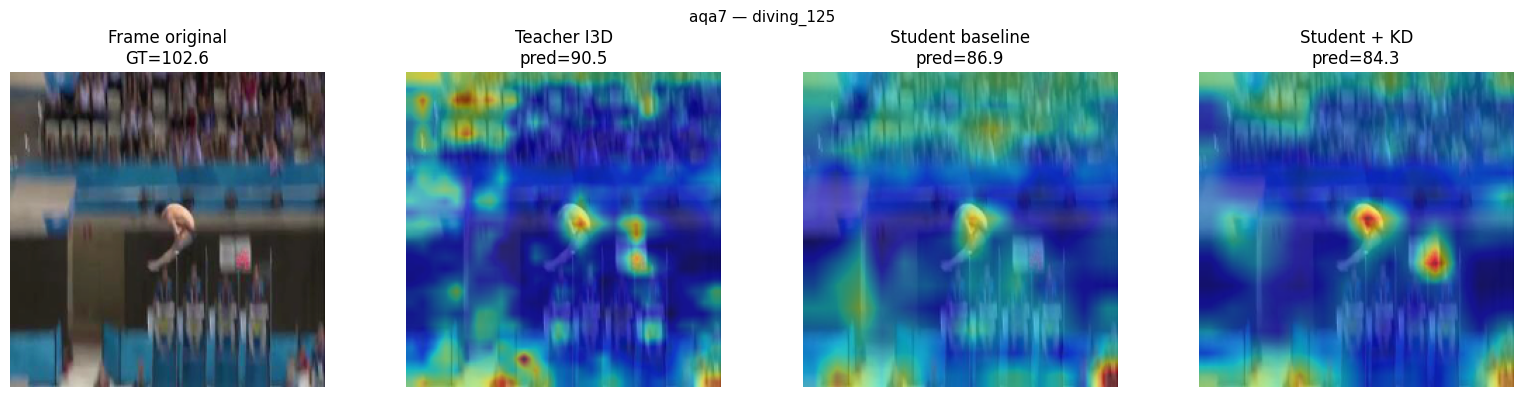
\includegraphics[width=0.85\textwidth]{figs/Resultados/gradcam_aqa7_diving.png} \\
        {\footnotesize (a) AQA-7 -- clavado (\textit{diving\_125})} \\[0.4em]
        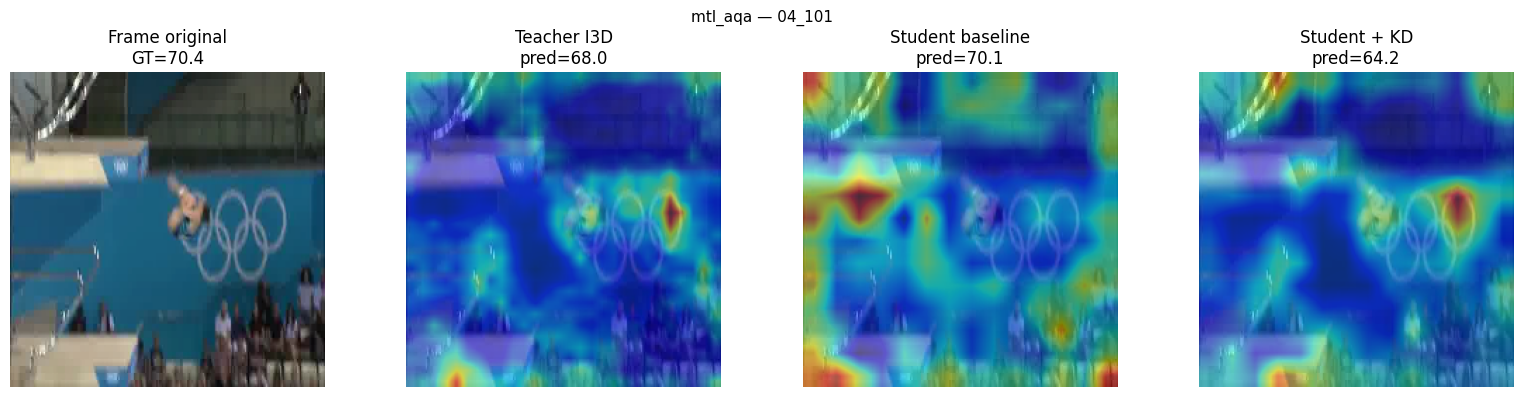
\includegraphics[width=0.85\textwidth]{figs/Resultados/gradcam_mtl_aqa.png} \\
        {\footnotesize (b) MTL-AQA -- clavado (04\_101)} \\[0.4em]
        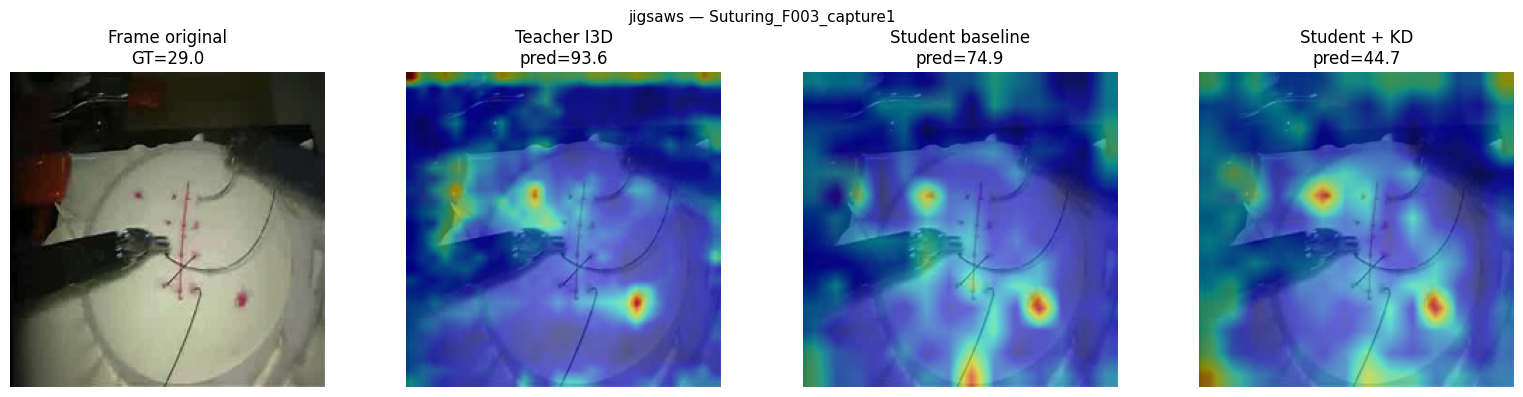
\includegraphics[width=0.85\textwidth]{figs/Resultados/gradcam_jigsaws_suturing.png} \\
        {\footnotesize (c) JIGSAWS -- \textit{Suturing} (F003, capture1)} \\
    \end{tabular}
    \caption{Mapas de atención Grad-CAM para Teacher (\ac{I3D}), \textit{pipeline} liviano y variante \textit{+~KD} en los tres dominios evaluados. En deportes, el \textit{Teacher} concentra la atención sobre el cuerpo del atleta durante la fase clave del movimiento; en cirugía, todos los modelos convergen sobre las manos y los instrumentos.}
    \label{fig:gradcam}
\end{figure}

La inspección visual muestra que el \textit{Teacher} \ac{I3D} concentra su atención sobre el cuerpo del atleta y las extremidades durante la fase clave del movimiento. El \textit{pipeline} liviano sin destilación reproduce patrones cualitativamente similares, lo cual es coherente con la pequeña brecha cuantitativa de \ac{SRCC}. En JIGSAWS las atenciones convergen sobre las manos del cirujano y los instrumentos, indicando que los modelos aprenden a localizar la región relevante incluso en un dominio radicalmente distinto al de pre-entrenamiento.
